\section{Radds存储系统总体设计}

	Radds存储系统总体架构组成如\Cref{overall_structure}所示,省略一段文字省略一段文字省略一段文字省略一段文字省略一段文字省略一段文字省略一段文字省略一段文字省略一段文字省略一段文字省略一段文字省略一段文字省略一段文字省
		
	\begin{figure}[H]
		\centering
		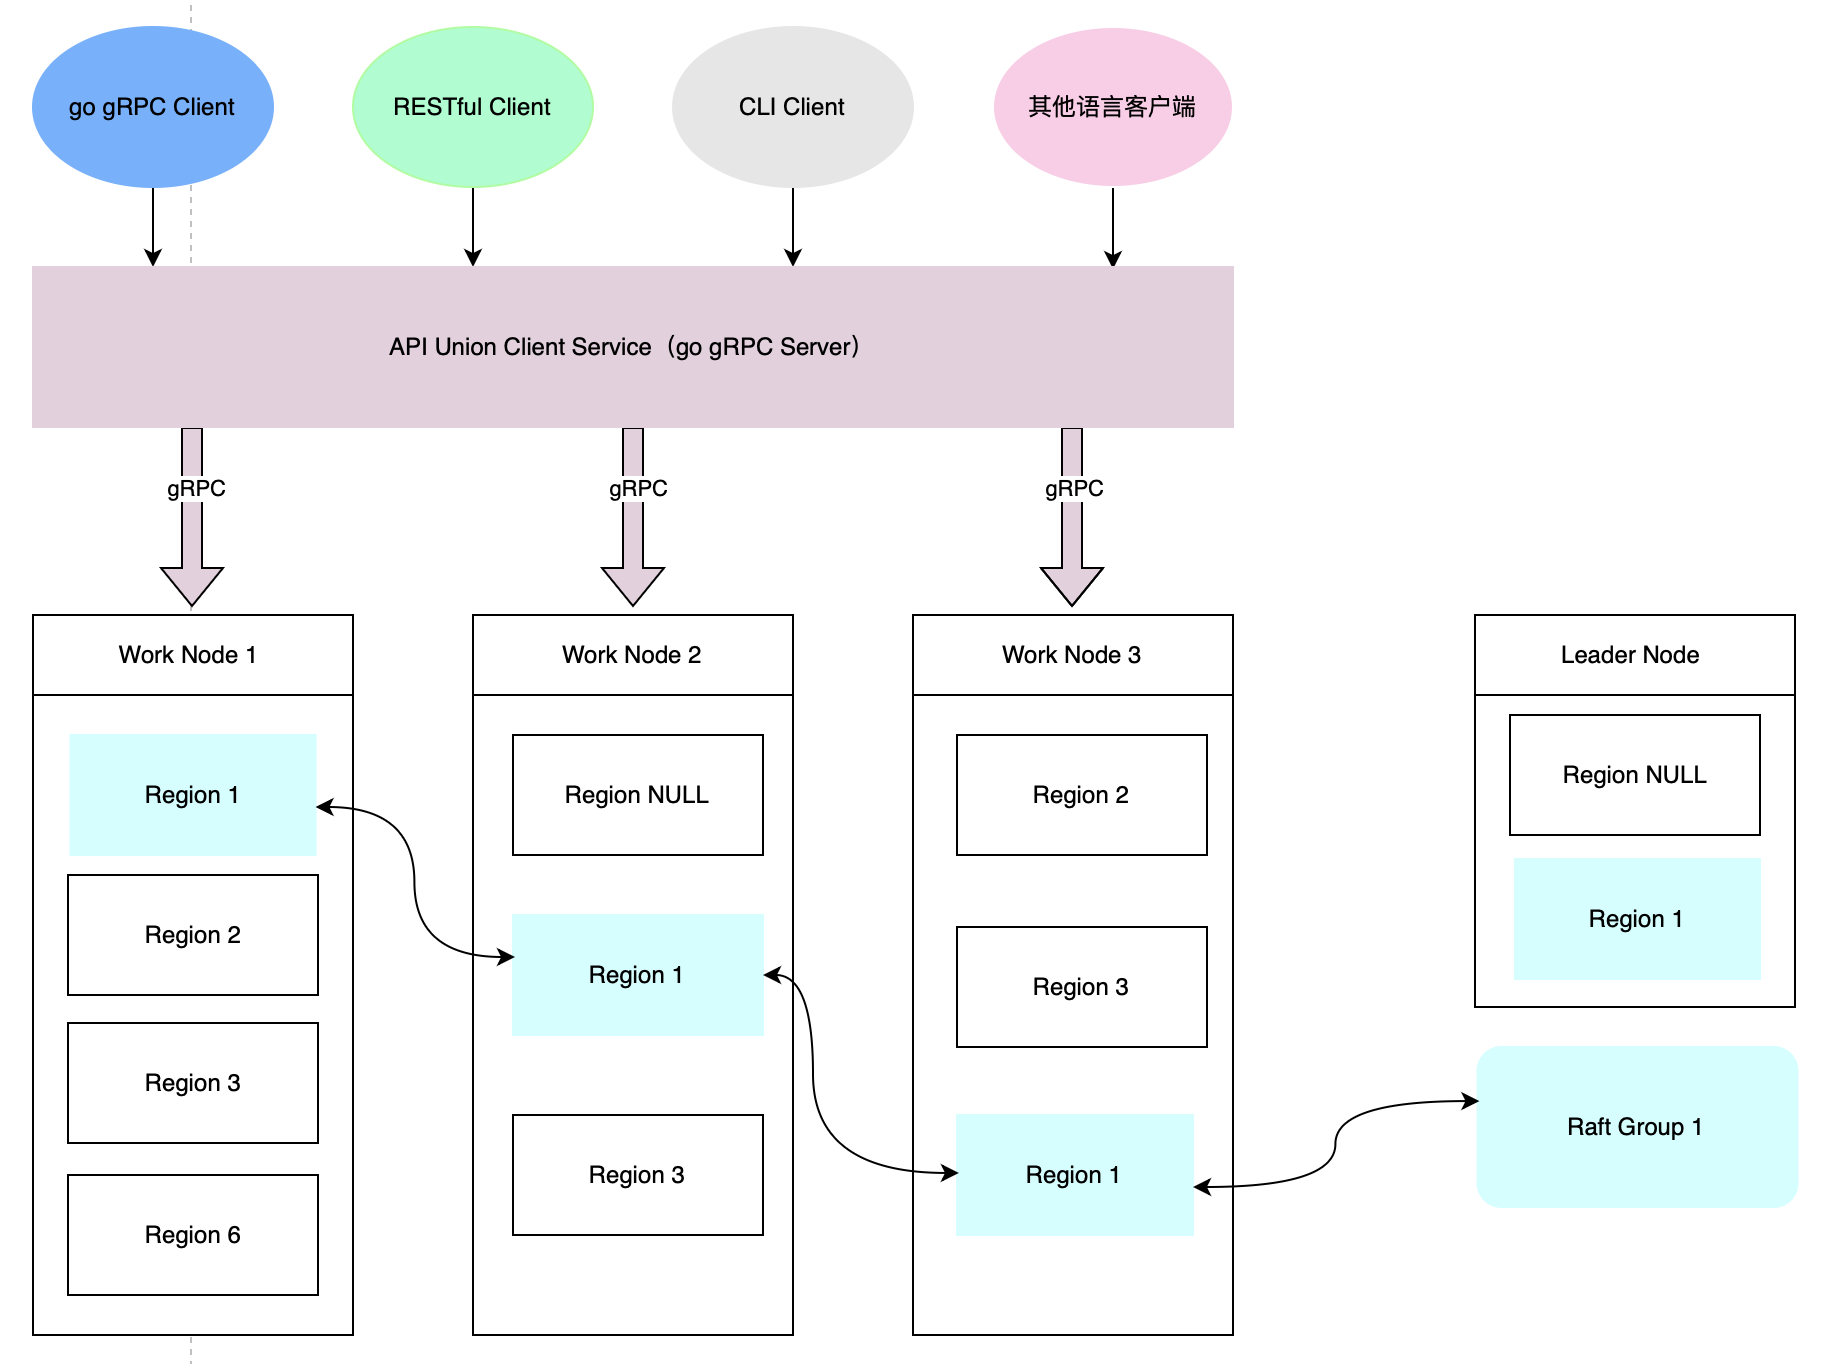
\includegraphics[width=0.80\textwidth]{images/radds_system_arch}
		\caption{Radds存储系统总体架构图}
		\label{overall_structure}
	\end{figure}
	
	\subsection{存储系统架构设计}
	
		服务端的实现省略一段文字省略一段文字省略一段文字省略一段文字省略一段文字省略一段文字省略一段文字省略一段文字省略一段文字省略一段文字省略一段文字省略一段文字省略一段文字省		  
		  
		 省略一段文字省略一段文字省略一段文字省略一段文字省略一段文字省略一段文字省略一段文字省略一段文字省略一段文字省略一段文字省略一段文字省略一段文字省略一段文字省
		 
		  		  
		  
	\subsection{存储层功能总体设计}
			
	\begin{figure}[H]
		\centering
		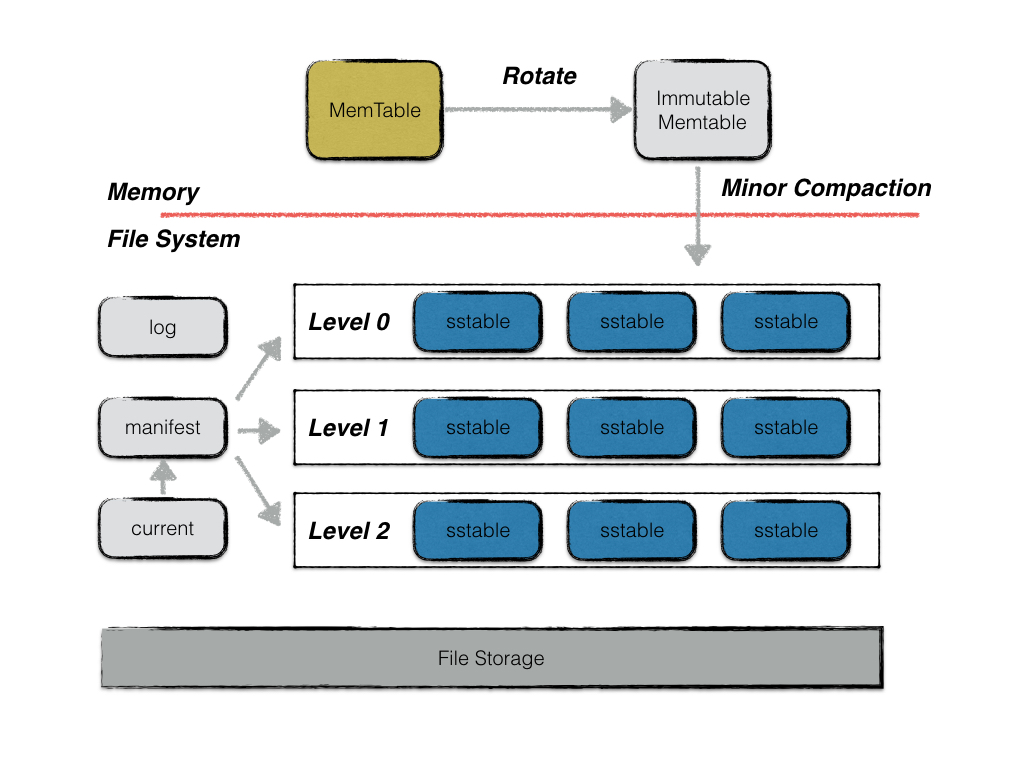
\includegraphics[width=0.95\textwidth]{images/radds_storage_arch}
		\caption{Radds存储层架构设计}
		\label{mobile_overall_design}
	\end{figure}


	\begin{enumerate}[fullwidth,itemindent=2em,listparindent=2em]
	
		\item 存储引擎设计概述
		
		我们要实现一个写性能优秀的存储引擎,则必须实现一个LSM树(Log Structured-Merge Tree)实现。LSM树的核心思想就是放弃部分读的性能,换取最大的写入能力。

		LSM树写性能极高的原理,简单地来说就是尽量减少随机写的次数。对于每次写入操作,并不是直接将最新的数据驻留在磁盘中,而是将其拆分成
		(1){一次日志文件的顺序写}
		(2){一次内存中的数据插入}

		存储架构正是实践了这种思想,将数据首先更新在内存中,当内存中的数据达到一定的阈值,将这部分数据真正刷新到磁盘文件中,因而获得了极高的写性能(顺序写60MB/s, 随机写45MB/s)。

	\end{enumerate}
		\subsubsection{内存可变数据memtable总体设计}
		
		之前提到,存储引擎的一次写入操作并不是直接将数据刷新到磁盘文件,
		而是首先写入到内存中作为代替,memtable就是一个在内存中进行数据组织与维护的结构。
		memtable中,所有的数据按用户定义的排序方法排序之后按序存储,
		等到其存储内容的容量达到阈值时(默认为4MB),便将其转换成一个不可修改的memtable,
		与此同时创建一个新的memtable,供用户继续进行读写操作。
		memtable底层使用了一种跳表数据结构\scite{cite_skiplist},这种数据结构效率可以比拟二叉查找树,
		绝大多数操作的时间复杂度为O(log n)。

		\subsubsection{内存不可变数据immutable memtable总体设计}

		memtable的容量到达阈值时,便会转换成一个不可修改的memtable,
		也称为immutable memtable。这两者的结构定义完全一样,
		区别只是immutable memtable是只读的。
		当一个immutable memtable被创建时,存储系统的后台压缩进程便会将利用其中的内容,
		创建一个sstable,持久化到磁盘文件中。

		\subsubsection{日志文件journal总体设计}

		存储系统的写操作并不是直接写入磁盘的,而是首先写入到内存。
		假设写入到内存的数据还未来得及持久化,存储系统进程发生了异常,抑或是宿主机器发生了宕机,
		会造成用户的写入发生丢失。因此存储系统在写内存之前会首先将所有的写操作写到日志文件中,
		也就是log文件。当以下异常情况发生时,均可以通过日志文件进行恢复:

		\begin{enumerate}
			\item 写log期间进程异常;
			\item 写log完成,写内存未完成;
			\item write动作完成(即log、内存写入都完成)后,进程异常;
			\item immutable memtable持久化过程中进程异常;
			\item 其他压缩异常(较为复杂,首先不在这里介绍);
		\end{enumerate}
	
	异常发生时,处理的情况分两种:
		\begin{enumerate}
			\item 当第一类情况发生时,数据库重启读取log时,
			发现异常日志数据,抛弃该条日志数据,即视作这次用户写入失败,保障了数据库的一致性;
			\item 当第二类,第三类,第四类情况发生了,均可以通过redo日志文件中记录的写入操作完成数据库的恢复。
		\end{enumerate}
		每次日志的写操作都是一次顺序写,因此写效率高,整体写入性能较好。
		此外,存储系统的用户写操作的原子性同样通过日志来实现。

		\subsubsection{磁盘持久化sstable总体设计}

		虽然存储系统采用了先写内存的方式来提高写入效率,但是内存中数据不可能无限增长,
		且日志中记录的写入操作过多,会导致异常发生时,恢复时间过长。
		因此内存中的数据达到一定容量,就需要将数据持久化到磁盘中。
		除了某些元数据文件,存储系统的数据主要都是通过sstable来进行存储。

		虽然在内存中,所有的数据都是按序排列的,但是当多个memetable数据持久化到磁盘后,
		对应的不同的sstable之间是存在交集的,在读操作时,需要对所有的sstable文件进行遍历,
		严重影响了读取效率。因此leveldb后台会“定期“整合这些sstable文件,
		该过程也称为compaction。随着compaction的进行,sstable文件在逻辑上被分成若干层,
		由内存数据直接dump出来的文件称为level 0层文件,后期整合而成的文件为level i 层文件,
		这也是以leveldb为原型的存储系统的这个名字的由来。

		注意,所有的sstable文件本身的内容是不可修改的,这种设计哲学为leveldb带来了许多优势,
		简化了很多设计。

		\subsubsection{文件元数据manifest总体设计}

		存储系统中有个版本的概念,一个版本中主要记录了每一层中所有文件的元数据,
		元数据包括(1)文件大小(2)最大key值(3)最小key值。
		该版本信息十分关键,除了在查找数据时,利用维护的每个文件的最大/小key值来加快查找,
		还在其中维护了一些进行compaction的统计值,来控制compaction的进行。

		一个文件的元数据主要包括了最大最小key,文件大小等信息;\Cref{code_radds_storage_tfile}
		
		\begin{lstlisting}[caption=tFile , label=code_radds_storage_tfile]
			type tFile struct {
    			fd         storage.FileDesc
    			seekLeft   int32
    			size       int64
    			imin, imax internalKey
			}
		\end{lstlisting}

		\subsubsection{版本号current总体设计}

		一个版本信息主要维护了每一层所有文件的元数据。
		\begin{lstlisting}[caption=tFile , label=code_radds_storage_tfile]
		type version struct {
    		s *session // session - version
    		levels []tFiles // file meta
    		cLevel int // next level
    		cScore float64 // current score
    		cSeek unsafe.Pointer
    		closing  bool
    		ref      int
    		released bool
		}
		\end{lstlisting}

		当每次compaction完成(或者换一种更容易理解的说法,当每次sstable文件有新增或者减少),l
		eveldb都会创建一个新的version,创建的规则是:

		versionNew = versionOld + versionEdit

		versionEdit指代的是基于旧版本的基础上,变化的内容(例如新增或删除了某些sstable文件)。

		manifest文件就是用来记录这些versionEdit信息的。
		一个versionEdit数据,会被编码成一条记录,写入manifest文件中。
		如\Cref{radds_storage_manifest}便是一个manifest文件的示意图,其中包含了3条versionEdit记录,
		每条记录包括(1)新增哪些sst文件(2)删除哪些sst文件(3)当前compaction的下标
		(4)日志文件编号(5)操作seqNumber等信息。通过这些信息,leveldb便可以在启动时,
		基于一个空的version,不断apply这些记录,最终得到一个上次运行结束时的版本信息。

		\begin{figure}[H]
			\centering
			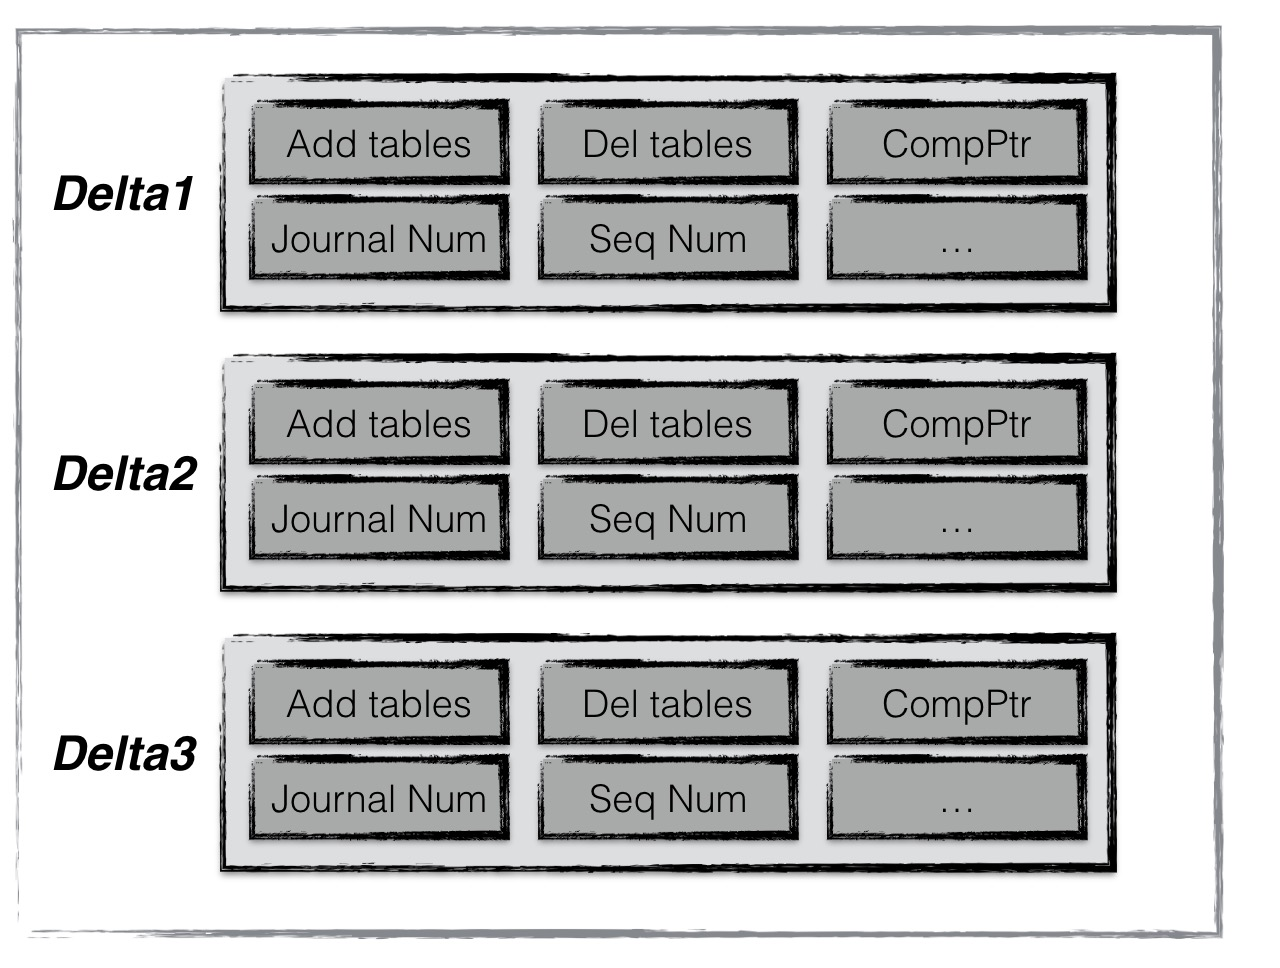
\includegraphics[width=0.80\textwidth]{images/manifest}
			\caption{版本信息记录数据结构}
			\label{radds_storage_manifest}
		\end{figure}

	\subsection{共识层功能总体设计}

		
		省略一段文字省略一段文字省略一段文字省略一段文字省略一段文字省略一段文字省略一段文字省略一段文字省略一段文字省略一段文字省略一段文字省,表格使用,表格使用,表格使用,表格使用,表格使用,表格使用,如\Cref{tab:db_table_user}所示。
	
		\begin{table}[H]
		\centering
		\caption{User 用户表}
		\zihao{5}
		\label{tab:db_table_user}
		\begin{tabular}{p{0.21\textwidth}p{0.21\textwidth}p{0.21\textwidth}p{0.21\textwidth}}
		\hline
		字段          & 数据类型         & 字段含义   & 约束条件     \\ \hline
		id          & INT(11)      & 用户ID & 主键、非空、自增 \\
		im\_id      & VARCHAR(256) & 环信ID & 唯一       \\ 
		account     & VARCHAR(45)  & 用户名  & 唯一       \\ 
		nick\_name  & VARCHAR(100) & 昵称   & 无        \\
		password    & VARCHAR(256) & 密码   & 非空       \\ 
		email       & VARCHAR(45)  & 邮箱   & 无        \\
		mobile      & VARCHAR(45)  & 手机号  & 唯一        \\ 
		sex         & INT(11)      & 性别   & 无        \\ 
		signature   & VARCHAR(512) & 签名   & 无        \\
		avatar      & VARCHAR(256) & 头像   & 无        \\
		is\_deleted & TINYINT(4)   & 删除标志 & 无        \\ \hline
		\end{tabular}
		\end{table}
	

	\subsection{客户端功能总体设计}
	
	\subsubsection{gRPC API客户端总体设计}
	\subsubsection{RESTful API客户端总体设计}
	\subsubsection{CLI 客户端总体设计}
	\subsection{本章小结}
	
 \clearpage